We conducted a user study of \evantodo{NUMBER} participants to determine if
there is a statistically significant difference among users in
performing certain tasks on repositories between \textit{Linvis} and
either gitk or the command-line git interface. We were looking for
improvements in accuracy, time performance, and overall enjoyment among
users when performing summarization and intra-tree navigation, as these
are the tasks that merge-trees are design to simplify.

\evan{still need to figure out who our intended user is... ``git user''
  is a bit too broad.}

% TODO: Determine who the intended user is. "generic git user" is kind of broad.
% TODO: Add a note stating that we will refer to the primary branch as being the master branch

\subsubsection{Methodology}
\label{ssub:methodology}

\subsubsection{Commit Selection}
\label{ssub:commit_selection}

We selected two commits for the participant to draw and summarize by
first determining the size of tree in the first and second quartiles. We
found that between Linux 3.1 and 3.16, the size of the trees in the
first quartile only contained a single node, and that the size of the
trees in the second quartile resulted in trees up to seven nodes. The
third quartile contained trees up to 51 nodes, and the fourth quartile
contained one tree of 7217 nodes. It is worth mentioning that the tree
sizes in the fourth quartile increase very quickly, as the next largest
tree only contains 4708 nodes, and the third largest tree contains 2349
commits. We see in figure~\ref{fig:tree_size} how the number of trees
decreases as the size of the tree increases. The results for the other
plots become very noisy, since there is only one occurrence for any tree
with more than 947 commits, and only two occurrences of any trees with
size greater than 336. Due to the noise,
figures~\ref{fig:tree_size_filter},~\ref{fig:merge_count_filter},
and~\ref{fig:percentage_filter} are only on the sizes of trees where
there were at least three occurrences of trees of that size.

\pgfplotstableread[col sep=comma]{data/comdate_merge_size.csv}\comtable

\begin{figure}[htpb]
  \centering
  \begin{tikzpicture}
    \begin{axis} [
      ylabel=Tree size,
      xlabel=Date,
      grid=both
      ]
      \addplot[chartpurple] table[x index=1, y index=2]\comtable;
    \end{axis}
  \end{tikzpicture}

  \caption{Merge-tree size by date}
  \label{fig:}
\end{figure}

\pgfplotstableread[col sep=comma]{data/merge_counts.csv}\mergetable

\begin{figure}
  \centering
  \begin{tikzpicture}
    \begin{axis}[
      ylabel=Occurences,
      xlabel=Total Commits,
      grid=both,
      minor x tick num = 1,
      minor y tick num = 1
      ]
      \addplot[chartblue] table[col sep=comma, x index=1, y index=0]{data/tree_size.csv};
    \end{axis}
  \end{tikzpicture}
  \caption{Frequency of trees of varying sizes}
  \label{fig:tree_size}
\end{figure}

\begin{figure}
  \centering
  \begin{tikzpicture}
    \begin{axis}[
      ylabel=Occurences,
      xlabel=Total Commits,
      grid=both,
      minor x tick num = 1,
      minor y tick num = 1
      ]
      \addplot[chartblue] table[x index=0, y index=1]\mergetable;
    \end{axis}
  \end{tikzpicture}
  \caption{Frequency of trees of varying sizes}
  \label{fig:tree_size_filter}
\end{figure}

\begin{figure}[htpb]
  \centering
  \begin{tikzpicture}
    \begin{axis} [
      ylabel=Merges,
      xlabel=Total Commits,
      minor x tick num = 1,
      minor y tick num = 1,
      grid=both,
      legend pos = north west
      ]
      \addplot[chartred] table[x index=0, y index=5]\mergetable;
      \addlegendentry{Maximum}
      \addplot[chartyellow] table[x index=0, y index=6]\mergetable;
      \addlegendentry{Mean}
      \addplot[chartgreen] table[x index=0, y index=4]\mergetable;
      \addlegendentry{Median}
      \addplot[chartblue] table[x index=0, y index=3]\mergetable;
      \addlegendentry{Minimum}
    \end{axis}
  \end{tikzpicture}
  \caption{Number of merges versus the size of the merge tree}
  \label{fig:merge_count_filter}
\end{figure}

\begin{figure}[htpb]
  \centering
  \begin{tikzpicture}
    \begin{axis} [
      ylabel=Merge Percentage,
      xlabel=Total Commits,
      grid=both
      ]
      \addplot[chartpurple] table[x index=0, y index=7]\mergetable;
    \end{axis}
  \end{tikzpicture}
  \caption{Percentage of commits in a merge-tree that are merge commits}
  \label{fig:percentage_filter}
\end{figure}

As 25\% of the trees consist of a single commit, we selected one tree
consisting of a single commit for the study. 50\% of the trees contained
up to seven nodes, so we selected another tree of size seven.  Of these
trees, we restricted the selection to trees consisting of at least one
merge, not including the merge into the master branch.

From the list of trees consisting of a single node, we selected one at
random using the \verb|random.choice()| function in python 3.6.1, which
returned the merge tree rooted at
\emph{11df5864075f763ec0d1fdecd6a3f0af7d09a553}. As we are not testing
the inter-tree and tree-search capabilities of \emph{Linvis}, we start
the user at the corresponding commit. In this case, there is only a
single option, commit \emph{a3c1239eb59c0a907f8be5587d42e950f44543f8},
shown in Figure~\ref{fig:commit_1}.

\begin{figure}[htpb]
  \centering
  
\includegraphics[width=0.2\linewidth]{figures/commits/1-commit.pdf}
  \caption{The first merge tree used in the user study, a merge tree
    containing a single commit}
  \label{fig:commit_1}
\end{figure}

Using the same merge selection technique, we selected the tree rooted at
\emph{8eb88c80d444fd249edaa7d895666cde79e7b3b8}. To select the starting
commit, we use the python random choice function on the list of commit
hashes contained in this tree. This resulted in the selection of commit
\emph{cdbdd1676a5379f1d5cbd4d476f5e349f445befe}, shown in
Figure~\ref{fig:commit_2}.

\begin{figure}[htpb]
  \centering
  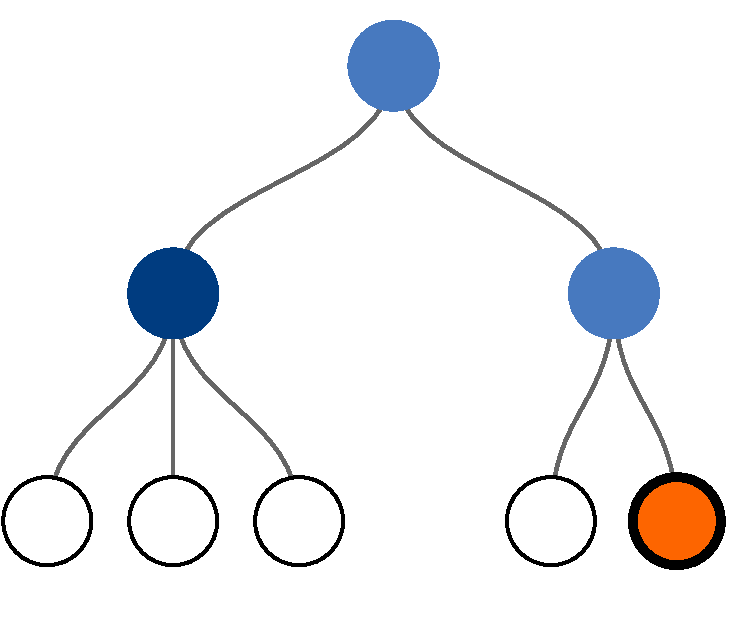
\includegraphics[width=0.5\linewidth]{figures/commits/7-commits.pdf}
  \caption{The second merge tree used in the user study, a merge tree
    containing seven commits}
  \label{fig:commit_2}
\end{figure}

\subsubsection{Questions}
\label{ssub:questions}

We chose questions that were designed to test the two primary goals of
merge trees, compared with the results from gitk or command line git.

The primary study questions are broken into two sections, one for
tree comprehension, and another section for summarization. A final
section is added, in order to have some information behind the
demographic of the participant.

\textbf{Conceptual Tasks}

As this information is provided directly by the \emph{Linvis} tree
visualizations, we use Gitk or git commandline for performing these
tasks.

\evan{Draw both trees, or just one tree?}
\begin{enumerate}
  \item Draw a diagram of the merge tree showing how the commit
    cdbdd1676a5379f1d5cbd4d476f5e349f445befe is merged into the master
    branch of the repository.
  \item How many individual commits are related to this commit?
  \item How many merges are involved with merging these commits into the
    master branch?
\end{enumerate}

We provide the user with 15 minutes to complete the first task, which is
to draw the diagram shown in Figure~\ref{fig:commit_2}. The other parts
of this task can be derived directly from the image drawn from the first
task. For this reason, we keep the ordering of these tasks consistent
between participants.

\textbf{Summarization Tasks}

We randomize the order of tool use, choosing to start with either
\emph{Linvis} or Gitk to ensure that information cannot be carried
forward from the previous tool across all participants.

The questions in this portion of the study are shuffled and presented in
random order, except where one task follows from another. We use the
\verb|random.shuffle()| function from python 3.6.1 for performing the
shuffling and presentation of the tasks.

We asked the following questions in randomized order
\begin{enumerate}
  \item What other commits are merged in the same merge
  \item What is the series of merges involved with merging this commit
  \item \label{it:aut1} How many authors are involved with this merge
  \item \label{it:aut2}Who contributed the most changes to this merge
  \item \label{it:f1}How many files were modified in this merge?
  \item \label{it:f2}Which files had the most changes in this merge?
  \item Which modules does this merge tree involve?
\end{enumerate}

We identify items \ref{it:aut1} and \ref{it:aut2} to be related,
concerning the authorship, and items \ref{it:f1} and \ref{it:f2} to be
related, concerning the files of a merge tree. The related items will be
in the same order consistently between participants, but the order of
tasks will be changed between participants.

\textbf{User Demographic}

This section of the study provides us with some information about our
participant, and how they felt about using gitk versus \emph{Linvis}.

We asked the following questions in this order
\begin{enumerate}
  \item Given these tasks again, which tool would you prefer to use?
  \item Which aspects of each tool did you like and why?
  \item How long have you used git?
  \item If you have used git, for what kind of projects? (personal,
    school courses, professional?)
  \item If you have used git, how many commits, files, and contributors
    were involved with the largest repository you have worked with?
\end{enumerate}

These questions will provide us with some information about how the user
felt, and their experience with git.

\subsubsection{Study}
\label{ssub:study}

The null hypothesis is that using merge trees or using the DAG directly
does not affect the performance of users.
